\documentclass{standalone}
\usepackage{tikz}
\usetikzlibrary{patterns, positioning}

\begin{document}
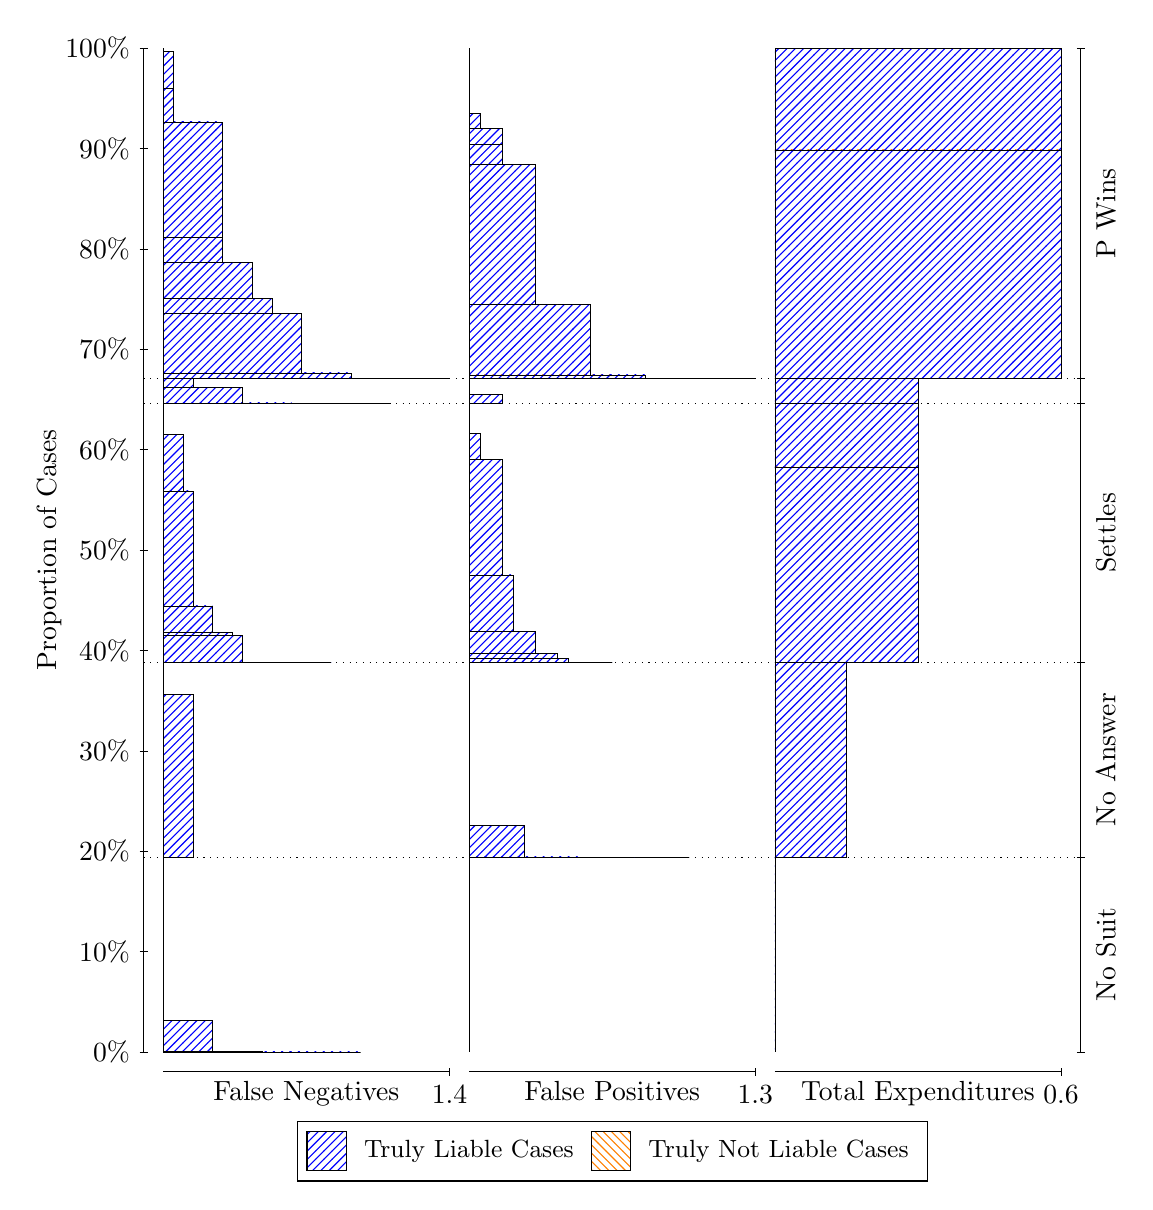
\begin{tikzpicture}
\draw[black, very thin] (1.5,1.75) -- (1.5,14.5);
\node[rotate=90, anchor=center] at (0.3, 8.125) {Proportion of Cases};
\draw[black, very thin] (1.45,1.75) -- (1.55,1.75);
\node[anchor=east] at (1.45, 1.75) {0\%};
\draw[black, very thin] (1.45,3.025) -- (1.55,3.025);
\node[anchor=east] at (1.45, 3.025) {10\%};
\draw[black, very thin] (1.45,4.3) -- (1.55,4.3);
\node[anchor=east] at (1.45, 4.3) {20\%};
\draw[black, very thin] (1.45,5.575) -- (1.55,5.575);
\node[anchor=east] at (1.45, 5.575) {30\%};
\draw[black, very thin] (1.45,6.85) -- (1.55,6.85);
\node[anchor=east] at (1.45, 6.85) {40\%};
\draw[black, very thin] (1.45,8.125) -- (1.55,8.125);
\node[anchor=east] at (1.45, 8.125) {50\%};
\draw[black, very thin] (1.45,9.4) -- (1.55,9.4);
\node[anchor=east] at (1.45, 9.4) {60\%};
\draw[black, very thin] (1.45,10.675) -- (1.55,10.675);
\node[anchor=east] at (1.45, 10.675) {70\%};
\draw[black, very thin] (1.45,11.95) -- (1.55,11.95);
\node[anchor=east] at (1.45, 11.95) {80\%};
\draw[black, very thin] (1.45,13.225) -- (1.55,13.225);
\node[anchor=east] at (1.45, 13.225) {90\%};
\draw[black, very thin] (1.45,14.5) -- (1.55,14.5);
\node[anchor=east] at (1.45, 14.5) {100\%};

\draw[black, very thin] (13.4,1.75) -- (13.4,14.5);
\draw[black, very thin] (13.35,1.75) -- (13.45,1.75);
\node[anchor=west] at (13.35, 1.75) {};
\draw[black, very thin] (13.35,4.2243) -- (13.45,4.2243);
\node[anchor=west] at (13.35, 4.2243) {};
\draw[black, very thin] (13.35,6.6985) -- (13.45,6.6985);
\node[anchor=west] at (13.35, 6.6985) {};
\draw[black, very thin] (13.35,9.9872) -- (13.45,9.9872);
\node[anchor=west] at (13.35, 9.9872) {};
\draw[black, very thin] (13.35,10.302) -- (13.45,10.302);
\node[anchor=west] at (13.35, 10.302) {};
\draw[black, very thin] (13.35,14.5) -- (13.45,14.5);
\node[anchor=west] at (13.35, 14.5) {};

\draw[black, very thin, pattern color=blue, pattern=north east lines] (1.75,1.75) rectangle (4.2557,1.75);
\draw[black, very thin, pattern color=blue, pattern=north east lines] (1.75,1.75) rectangle (3.6293,1.75);
\draw[black, very thin, pattern color=blue, pattern=north east lines] (1.75,1.75) rectangle (3.0029,1.7535);
\draw[black, very thin, pattern color=blue, pattern=north east lines] (1.75,1.7535) rectangle (2.3764,2.1551);
\draw[black, very thin, pattern color=orange, pattern=north west lines] (1.75,2.1551) rectangle (1.75,2.1551);
\draw[black, very thin, pattern color=blue, pattern=north east lines] (1.75,2.1551) rectangle (1.75,4.2243);
\draw[black, very thin, pattern color=blue, pattern=north east lines] (1.75,4.2243) rectangle (2.1259,6.2933);
\draw[black, very thin, pattern color=orange, pattern=north west lines] (1.75,6.2933) rectangle (1.75,6.2933);
\draw[black, very thin, pattern color=blue, pattern=north east lines] (1.75,6.2933) rectangle (1.75,6.6985);
\draw[black, very thin, pattern color=blue, pattern=north east lines] (1.75,6.6985) rectangle (3.8799,6.6985);
\draw[black, very thin, pattern color=blue, pattern=north east lines] (1.75,6.6985) rectangle (3.6293,6.6985);
\draw[black, very thin, pattern color=blue, pattern=north east lines] (1.75,6.6985) rectangle (3.3787,6.6992);
\draw[black, very thin, pattern color=blue, pattern=north east lines] (1.75,6.6992) rectangle (3.2534,6.6992);
\draw[black, very thin, pattern color=blue, pattern=north east lines] (1.75,6.6992) rectangle (3.0029,6.7021);
\draw[black, very thin, pattern color=blue, pattern=north east lines] (1.75,6.7021) rectangle (2.7523,7.04);
\draw[black, very thin, pattern color=blue, pattern=north east lines] (1.75,7.04) rectangle (2.627,7.0779);
\draw[black, very thin, pattern color=blue, pattern=north east lines] (1.75,7.0779) rectangle (2.3764,7.4148);
\draw[black, very thin, pattern color=blue, pattern=north east lines] (1.75,7.4148) rectangle (2.1259,8.8771);
\draw[black, very thin, pattern color=blue, pattern=north east lines] (1.75,8.8771) rectangle (2.0006,9.5922);
\draw[black, very thin, pattern color=orange, pattern=north west lines] (1.75,9.5922) rectangle (1.75,9.5922);
\draw[black, very thin, pattern color=blue, pattern=north east lines] (1.75,9.5922) rectangle (1.75,9.9872);
\draw[black, very thin, pattern color=blue, pattern=north east lines] (1.75,9.9872) rectangle (4.6316,9.9872);
\draw[black, very thin, pattern color=blue, pattern=north east lines] (1.75,9.9872) rectangle (4.0052,9.9872);
\draw[black, very thin, pattern color=blue, pattern=north east lines] (1.75,9.9872) rectangle (3.3787,9.994);
\draw[black, very thin, pattern color=blue, pattern=north east lines] (1.75,9.994) rectangle (2.7523,10.191);
\draw[black, very thin, pattern color=blue, pattern=north east lines] (1.75,10.191) rectangle (2.1259,10.302);
\draw[black, very thin, pattern color=orange, pattern=north west lines] (1.75,10.302) rectangle (1.75,10.302);
\draw[black, very thin, pattern color=blue, pattern=north east lines] (1.75,10.302) rectangle (5.3833,10.302);
\draw[black, very thin, pattern color=blue, pattern=north east lines] (1.75,10.302) rectangle (4.7569,10.303);
\draw[black, very thin, pattern color=blue, pattern=north east lines] (1.75,10.303) rectangle (4.381,10.303);
\draw[black, very thin, pattern color=blue, pattern=north east lines] (1.75,10.303) rectangle (4.1305,10.374);
\draw[black, very thin, pattern color=blue, pattern=north east lines] (1.75,10.374) rectangle (3.7546,10.374);
\draw[black, very thin, pattern color=blue, pattern=north east lines] (1.75,10.374) rectangle (3.504,11.134);
\draw[black, very thin, pattern color=blue, pattern=north east lines] (1.75,11.134) rectangle (3.1282,11.318);
\draw[black, very thin, pattern color=blue, pattern=north east lines] (1.75,11.318) rectangle (2.8776,11.78);
\draw[black, very thin, pattern color=blue, pattern=north east lines] (1.75,11.78) rectangle (2.5017,12.098);
\draw[black, very thin, pattern color=blue, pattern=north east lines] (1.75,12.098) rectangle (2.5017,13.561);
\draw[black, very thin, pattern color=blue, pattern=north east lines] (1.75,13.561) rectangle (2.2511,13.561);
\draw[black, very thin, pattern color=blue, pattern=north east lines] (1.75,13.561) rectangle (1.8753,13.986);
\draw[black, very thin, pattern color=blue, pattern=north east lines] (1.75,13.986) rectangle (1.8753,14.454);
\draw[black, very thin, pattern color=orange, pattern=north west lines] (1.75,14.454) rectangle (1.75,14.454);
\draw[black, very thin, pattern color=blue, pattern=north east lines] (1.75,14.454) rectangle (1.75,14.5);
\draw[black, very thin, pattern color=orange, pattern=north west lines] (5.6333,1.75) rectangle (5.6333,1.75);
\draw[black, very thin, pattern color=blue, pattern=north east lines] (5.6333,1.75) rectangle (5.6333,4.2243);
\draw[black, very thin, pattern color=orange, pattern=north west lines] (5.6333,4.2243) rectangle (8.4282,4.2243);
\draw[black, very thin, pattern color=blue, pattern=north east lines] (5.6333,4.2243) rectangle (8.4282,4.2243);
\draw[black, very thin, pattern color=blue, pattern=north east lines] (5.6333,4.2243) rectangle (7.7295,4.2243);
\draw[black, very thin, pattern color=blue, pattern=north east lines] (5.6333,4.2243) rectangle (7.0308,4.2277);
\draw[black, very thin, pattern color=blue, pattern=north east lines] (5.6333,4.2277) rectangle (6.3321,4.6294);
\draw[black, very thin, pattern color=blue, pattern=north east lines] (5.6333,4.6294) rectangle (5.6333,6.6985);
\draw[black, very thin, pattern color=orange, pattern=north west lines] (5.6333,6.6985) rectangle (7.45,6.6985);
\draw[black, very thin, pattern color=blue, pattern=north east lines] (5.6333,6.6985) rectangle (7.45,6.6985);
\draw[black, very thin, pattern color=orange, pattern=north west lines] (5.6333,6.6985) rectangle (7.1705,6.6985);
\draw[black, very thin, pattern color=blue, pattern=north east lines] (5.6333,6.6985) rectangle (7.1705,6.6992);
\draw[black, very thin, pattern color=orange, pattern=north west lines] (5.6333,6.6992) rectangle (6.891,6.6992);
\draw[black, very thin, pattern color=blue, pattern=north east lines] (5.6333,6.6992) rectangle (6.891,6.7527);
\draw[black, very thin, pattern color=blue, pattern=north east lines] (5.6333,6.7527) rectangle (6.7513,6.8165);
\draw[black, very thin, pattern color=blue, pattern=north east lines] (5.6333,6.8165) rectangle (6.4718,7.0935);
\draw[black, very thin, pattern color=blue, pattern=north east lines] (5.6333,7.0935) rectangle (6.1923,7.8086);
\draw[black, very thin, pattern color=blue, pattern=north east lines] (5.6333,7.8086) rectangle (6.0526,9.2709);
\draw[black, very thin, pattern color=blue, pattern=north east lines] (5.6333,9.2709) rectangle (5.7731,9.6078);
\draw[black, very thin, pattern color=blue, pattern=north east lines] (5.6333,9.6078) rectangle (5.6333,9.9872);
\draw[black, very thin, pattern color=orange, pattern=north west lines] (5.6333,9.9872) rectangle (6.0526,9.9872);
\draw[black, very thin, pattern color=blue, pattern=north east lines] (5.6333,9.9872) rectangle (6.0526,10.098);
\draw[black, very thin, pattern color=blue, pattern=north east lines] (5.6333,10.098) rectangle (5.6333,10.302);
\draw[black, very thin, pattern color=orange, pattern=north west lines] (5.6333,10.302) rectangle (9.2667,10.302);
\draw[black, very thin, pattern color=blue, pattern=north east lines] (5.6333,10.302) rectangle (9.2667,10.302);
\draw[black, very thin, pattern color=orange, pattern=north west lines] (5.6333,10.302) rectangle (8.5679,10.302);
\draw[black, very thin, pattern color=blue, pattern=north east lines] (5.6333,10.302) rectangle (8.5679,10.302);
\draw[black, very thin, pattern color=orange, pattern=north west lines] (5.6333,10.302) rectangle (7.8692,10.302);
\draw[black, very thin, pattern color=blue, pattern=north east lines] (5.6333,10.302) rectangle (7.8692,10.348);
\draw[black, very thin, pattern color=orange, pattern=north west lines] (5.6333,10.348) rectangle (7.45,10.348);
\draw[black, very thin, pattern color=blue, pattern=north east lines] (5.6333,10.348) rectangle (7.45,10.348);
\draw[black, very thin, pattern color=orange, pattern=north west lines] (5.6333,10.348) rectangle (7.1705,10.348);
\draw[black, very thin, pattern color=blue, pattern=north east lines] (5.6333,10.348) rectangle (7.1705,11.241);
\draw[black, very thin, pattern color=orange, pattern=north west lines] (5.6333,11.241) rectangle (6.7513,11.241);
\draw[black, very thin, pattern color=blue, pattern=north east lines] (5.6333,11.241) rectangle (6.7513,11.241);
\draw[black, very thin, pattern color=blue, pattern=north east lines] (5.6333,11.241) rectangle (6.4718,13.022);
\draw[black, very thin, pattern color=blue, pattern=north east lines] (5.6333,13.022) rectangle (6.0526,13.275);
\draw[black, very thin, pattern color=orange, pattern=north west lines] (5.6333,13.275) rectangle (6.0526,13.275);
\draw[black, very thin, pattern color=blue, pattern=north east lines] (5.6333,13.275) rectangle (6.0526,13.484);
\draw[black, very thin, pattern color=blue, pattern=north east lines] (5.6333,13.484) rectangle (5.7731,13.668);
\draw[black, very thin, pattern color=blue, pattern=north east lines] (5.6333,13.668) rectangle (5.6333,14.5);
\draw[black, very thin, pattern color=orange, pattern=north west lines] (9.5167,1.75) rectangle (9.5167,1.75);
\draw[black, very thin, pattern color=blue, pattern=north east lines] (9.5167,1.75) rectangle (9.5167,4.2243);
\draw[black, very thin, pattern color=orange, pattern=north west lines] (9.5167,4.2243) rectangle (10.425,4.2243);
\draw[black, very thin, pattern color=blue, pattern=north east lines] (9.5167,4.2243) rectangle (10.425,6.6985);
\draw[black, very thin, pattern color=orange, pattern=north west lines] (9.5167,6.6985) rectangle (11.333,6.6985);
\draw[black, very thin, pattern color=blue, pattern=north east lines] (9.5167,6.6985) rectangle (11.333,9.1808);
\draw[black, very thin, pattern color=orange, pattern=north west lines] (9.5167,9.1808) rectangle (11.333,9.1808);
\draw[black, very thin, pattern color=blue, pattern=north east lines] (9.5167,9.1808) rectangle (11.333,9.9872);
\draw[black, very thin, pattern color=orange, pattern=north west lines] (9.5167,9.9872) rectangle (11.333,9.9872);
\draw[black, very thin, pattern color=blue, pattern=north east lines] (9.5167,9.9872) rectangle (11.333,10.302);
\draw[black, very thin, pattern color=orange, pattern=north west lines] (9.5167,10.302) rectangle (13.15,10.302);
\draw[black, very thin, pattern color=blue, pattern=north east lines] (9.5167,10.302) rectangle (13.15,13.206);
\draw[black, very thin, pattern color=orange, pattern=north west lines] (9.5167,13.206) rectangle (13.15,13.206);
\draw[black, very thin, pattern color=blue, pattern=north east lines] (9.5167,13.206) rectangle (13.15,14.5);
\draw[black, dotted] (1.5,4.2243) -- (13.4,4.2243);
\draw[black, dotted] (1.5,6.6985) -- (13.4,6.6985);
\draw[black, dotted] (1.5,9.9872) -- (13.4,9.9872);
\draw[black, dotted] (1.5,10.302) -- (13.4,10.302);
\draw[black, very thin] (1.75,1.5) -- (5.3833,1.5);
\node[anchor=north] at (3.5667, 1.5) {False Negatives};
\draw[black, very thin] (5.3833,1.45) -- (5.3833,1.55);
\node[anchor=north] at (5.3833, 1.45) {1.4};

\draw[black, very thin] (5.6333,1.5) -- (9.2667,1.5);
\node[anchor=north] at (7.45, 1.5) {False Positives};
\draw[black, very thin] (9.2667,1.45) -- (9.2667,1.55);
\node[anchor=north] at (9.2667, 1.45) {1.3};

\draw[black, very thin] (9.5167,1.5) -- (13.15,1.5);
\node[anchor=north] at (11.333, 1.5) {Total Expenditures};
\draw[black, very thin] (13.15,1.45) -- (13.15,1.55);
\node[anchor=north] at (13.15, 1.45) {0.6};

\node[black, centered, rotate=90] at (13.72, 2.9871) {No Suit};
\node[black, centered, rotate=90] at (13.72, 5.4614) {No Answer};
\node[black, centered, rotate=90] at (13.72, 8.3429) {Settles};

\node[black, centered, rotate=90] at (13.72, 12.401) {P Wins};

\draw (7.449999999999999,1.5) node[draw=none] (baseCoordinate) {};
\begin{scope}[align=center]
        \matrix[scale=0.5, draw=black, below=0.5cm of baseCoordinate, nodes={draw}, column sep=0.1cm]{
            \node[rectangle, draw, minimum width=0.5cm, minimum height=0.5cm, pattern=north east lines, pattern color=blue] {}; &
            \node[draw=none, font=\small] (B) {Truly Liable Cases}; &
            \node[rectangle, draw, minimum width=0.5cm, minimum height=0.5cm, pattern=north west lines, pattern color=orange] {}; &
            \node[draw=none, font=\small] (B) {Truly Not Liable Cases}; \\
            };
\end{scope}

\end{tikzpicture}
\end{document}